%  This LaTeX template is based on T.J. Hitchman's work which is itself based on Dana Ernst's template.  
% 
% --------------------------------------------------------------
% Skip this stuff, and head down to where it says "Start here"
% --------------------------------------------------------------
 
\documentclass[12pt]{article}
 \let\biconditional\leftrightarrow
\usepackage{tikz}
\usepackage[margin=1in]{geometry} 
\usepackage{amsmath,amsthm,amssymb}
\usetikzlibrary{arrows}
\theoremstyle{definition}

\newenvironment{definition}{\vspace{1em}\noindent\textbf{Definition.}}{\vspace{1em}}
%\usepackage{graphicx}
\newenvironment{statement}[2][Section]{\begin{trivlist}
\item[\hskip \labelsep {\bfseries #1}\hskip \labelsep {\bfseries #2.}]}{\end{trivlist}}

\begin{document}
\newtheorem{theorem}{Theorem} 
% --------------------------------------------------------------
%
%                         Start here
%
% --------------------------------------------------------------
 
\title{Analysis Done Right. (title w.i.p.)} % replace with the problem you are writing up
\author{Esteban Morales} % replace with your name
\maketitle


\begin{statement}{Chapter 1} %You can use theorem, exercise, problem, or question here.  Modify x.yz to be whatever number you are proving

Insert motivation ex. 1 (bolzanos existence problem)

Mathematicians wanted a way to show that there is an existence even if we do not have a 
direct way of finding.






\end{statement}
 
\begin{statement}{Absolute Value and Why it's so useful}


We will begin by describing the properties of absolute value as a refresher and a warm up 
to some "baby" proofs. \vspace{10pt}

The absolute value function is critical in our study of analysis as it is the first way that we will define a distance metric in one dimensional space. But more on distance later.


1.) Positive Definite.
$ \mid x \mid \ge 0$ and $ \mid x \mid= 0 \iff x = 0$\\


This first property is quite useful as it makes sure that our result will never be negative, which is extremely important when taking distance into consideration as negative distance has no inherent meaning.\\



2.) Multiplicative Property.
$\mid x * y \mid = \mid x \mid * \mid y \mid $
Multiplication works nicely with absolute value.\\

3.) Symmetry Property.
$\mid x \mid = \mid -x \mid$ \\
This property is a consequence of the positive definiteness property and is useful in some of the forthcoming proofs.\\

Corollary(with a short proof):
$\mid a - b \mid = \mid - (a - b) \mid = \mid b - a \mid \Rightarrow$\\
$\mid a - b \mid = \mid b - a \mid $\\
This corollary shows us that order is not important when subtracting inside the absolute value.\\

4.) Triangle Innequality
$\mid a + b \mid \le \mid a \mid + \mid b \mid$\\
A useful result that will help us with almost all of our limit proofs in the upcoming chapter.\\


5.) Second Definition
$\mid x \mid = \sqrt{x^2}$  \\

"Or $ \mid x \mid = \sqrt[n]{x} $ where $ n = 2k, k \in \mathbb{Z} $

"
6. Disjunctive Innequality 
let $ k > 0, \mid x \mid \ge k \iff x \ge k \vee x \le -k$\\
Take this example for k = 1 to help visualize the range of possibilites of x.\\

let $\mid x \mid \ge 1$



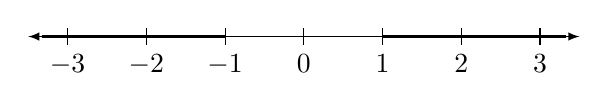
\begin{tikzpicture}
\draw[latex-latex] (-3.5,0) -- (3.5,0) ; %edit here for the axis
\foreach \x in  {-3,-2,-1,0,1,2,3} % edit here for the vertical lines
\draw[shift={(\x,0)},color=black] (0pt,3pt) -- (0pt,-3pt);
\foreach \x in {-3,-2,-1,0,1,2,3} % edit here for the numbers
\draw[shift={(\x,0)},color=black] (0pt,0pt) -- (0pt,-3pt) node[below] 
{$\x$};
\draw[very thick] (-3.33,0) -- (-1,0);
\draw[very thick] (1,0) -- (3.33,0);

\end{tikzpicture}\\




7.) Conjunctive Innequality
let $k > 0 \mid x \mid \le k \iff x > -k \land x < k $\\
Take another example where k = 2\\
Consider $\mid x \mid \le 2$\\

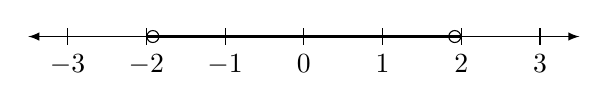
\begin{tikzpicture}
\draw[latex-latex] (-3.5,0) -- (3.5,0) ; %edit here for the axis
\foreach \x in  {-3,-2,-1,0,1,2,3} % edit here for the vertical lines
\draw[shift={(\x,0)},color=black] (0pt,3pt) -- (0pt,-3pt);
\foreach \x in {-3,-2,-1,0,1,2,3} % edit here for the numbers
\draw[shift={(\x,0)},color=black] (0pt,0pt) -- (0pt,-3pt) node[below] 
{$\x$};
\draw[very thick] (-2,0) -- (2,0);
\draw[-o] (-2,0) -- (2.,0);
\draw[o-] (-2,0) -- (2.,0);

\end{tikzpicture}\\








8. Division Property.
$\mid \frac{a}{b} \mid = \frac{\mid a \mid}{\mid b \mid} $ where b $\ne 0$
Another useful property that we will use extensively in the following chapter.\\

9.Absorption
$\mid \mid x \mid \mid = \mid x \mid$\\
\begin{proof}
Take $\mid \mid x \mid \mid = \mid x \mid$, $since \mid x \mid \ge 0,$ by def.
\end{proof}

10. Exponential Property.
$\mid x^k \mid = \mid x \mid^{k} $\\



11.) Connectedness
let $k > 0, \mid x \mid = k \iff x = k \vee x = -k$\\


These are all the properties of absolute value that we are going to be using in this text. We will commence the following page with proofs for all of these properties which again will serve as a nice warmup for what's to come.



\end{statement}

\begin{proof}

  1.)\textbf{ Proof of Positive Definite} \\
Recall : $ \mid x \mid \ge 0$ and $ \mid x \mid= 0 \iff x = 0$\\

Case 1: assume $x \ge 0, so \mid x \mid = x $\\
Case 2: $x < 0 so \mid x \mid = -1 * x$ $ Thus \mid x \mid > 0 \Rightarrow \mid x \mid \ge 0$\\
Assume that $\mid x \mid = 0$ and show that $x = 0$\\
We will now prove the biconditional going in the forwards direction
Assume towards a contradiction that $x \ne 0$\\
Case 1:$ x > 0 then \mid x \mid = x > 0$\\
Case 2:$ x < 0 \Rightarrow \mid x \mid = -1 * x, where -1 * x > 0, thus \mid x \mid > 0$\\
Which contracts our assumption that $\mid x \mid = 0, thus x \nless 0$\\
Thus we have shown that $\mid x \mid = 0 \Rightarrow x = 0$\\
Reverse Direction of the biconditional \\
if $ if x = 0 \Rightarrow \mid x \mid = 0, by def.$
So our conjunction portion is true.

\end{proof}

\begin{proof}

2.) Proof for multiplicative property.\\
Recall : $\mid x * y \mid = \mid x \mid * \mid y \mid $\\
$\mid ab \mid = \mid a \mid * \mid b \mid a,b \in \mathbb{R}$

Case 1, one real (a or b) is zero. Without loss of generality, let a be zero.\\
thus, $\mid ab \mid = \mid 0 * b \mid = \mid 0 \mid = 0$\\
Case 2. They have different signs(a * b $<$ 0) Without loss of generality let a $<$ 0 and b $>$ 0.\\
$\mid a*b \mid =$ -1 * a * b since they have different signs, where$ -1 * a * b > 0$\\
Case 3: They both have the same sign (a * b $> 0$) Without loss of generality let a,b $< 0$
$\mid a * b \mid$ = -1 * -1 * a * b = a * b
\end{proof}
 
\begin{proof}
  3. \textbf{Proof of Symmetry.}\\
Recall : $\mid x \mid = \mid -x \mid$ \\
$\mid -x \mid = \mid -1 * x \mid = \mid -1 \mid * \mid x \mid $, by the multiplicative property.\\
$1 * \mid x \mid = \mid x \mid $\\

\end{proof}

\begin{proof}
Proof of Corrollary\\
$\mid a - b \mid = \mid -1 * (b - a) \mid = \mid b - a \mid$


\end{proof}
\begin{proof}
\textbf{4.) Triangle Innequality}\\
Recall : $\mid a \pm b \mid \le \mid a \mid + \mid b \mid$\\
Note : $\forall x, x \le \mid x \mid $ and $ x \ge -1 * \mid x \mid $\\
Let $a,b \in \mathbb{R}$ We can observe \\
$ -1 * \mid a \mid \le a \le \mid a \mid$\\
$ -1 * \mid b \mid \le b \le \mid b \mid$\\
if we sum these two compound innequalities we obtain:\\
$-\mid a \mid - \mid b \mid \le a + b \le \mid a \mid + \mid b \mid \Rightarrow -1(\mid a \mid + \mid b \mid) \le a + b \le \mid a \mid + \mid b \mid$\\
If we look closely we can see a resemblance to the conjunctive innequality. We can see that our "k" is $\mid a \mid + \mid b \mid $
Thus we can say that $\mid a + b \mid \le \mid a \mid + \mid b \mid $ This can be expanded upon to include $\mid a - b \mid \le \mid a \mid + \mid b \mid $ as we can use the 3.) Symmetry Property inside the left hand side of our inequality.

\end{proof}


5. Will not be proven as it is an equivalent definition of the absoulte value\\


\begin{proof}
   \textbf{6. Proof of the disjunctive innequality}
   let $k \in \mathbb{R+} $
$   \mid x \mid \le \iff x \ge \vee x \le -k$\\
   Forward Direction of Biconditional:\\
   Assume that $\mid x \mid \ge k $ and we need to show that $x \ge k \vee x \le -k $\\
   Case 1: Assume $ x \ge 0$ so $\mid x \mid = x$ and $\mid x \mid \ge k ,thus x \ge k$\\
   Case 2: Asuume $ x < 0$ so $\mid x \mid = -1 * x$ thus, $ \mid x \mid \ge k \Rightarrow -1 * x \ge k \Rightarrow x \le -k $\\
   Now we look at the backwards direction.\\
   Assume $x \ge k \vee x \le -k$ We need to show that $\mid x \mid \ge k $\\
   Case 1: $ x \ge k > 0 \Rightarrow \mid x \mid = x \ge k$\\
   Case 2: $x \le k < 0 \Rightarrow \mid x \mid = -1 * x \ge k \Rightarrow \mid x \mid \ge k$
   Since we have demonstrated that both implications are true, their conjunct must be true and we have proven the equivalence of the disjunctive innequality.



\end{proof}

\begin{proof}
  \textbf{7.) Conjunctive Innquality.}
Recall : let $k > 0 \mid x \mid \le k \iff x > -k \land x < k $\\
 
Since we have another biconditional statement, we will first prove the forwards direction\\
$\Rightarrow$\\
Case 1: assume $\mid x \mid \le k$ and $x \ge 0$\\
$x \ge 0 \Rightarrow x > -k$ by hypothesis, k is positive. Also $\mid x \mid = x$ but $ \mid x \mid \le k \Rightarrow x \le k$\\
so $ -k \le x \land x \le k$\\
Case 2: assume $x < 0$\\
$x < 0 \Rightarrow \mid x \mid = -1 * x$, but $\mid x \mid \le k \Rightarrow -1 * x \le k \Rightarrow -k \le x$\\
Note that since $x < 0 \Rightarrow x \le k $ since we assumed k to be positive.\\
Thus $x \le k \land x \ge -k $\\
Now we will prove the backwards direcition\\
$\Leftarrow$\\
Assume that $-k \le x \le k$ we need to show that $\mid x \mid \le k$\\
Case 1: assume that $x \ge 0$ thus $\mid x \mid = x \le k$ by hypothesis\\
Case 2: assume that $ x < 0$ so $\mid x \mid = -1 * x$. We know that $x \ge -k$ and consequently $\mid x \mid = -1*x \le k \Rightarrow \mid x \mid \le k$\\

Thus we have proved both directions of the biconditional.

\end{proof}

\begin{proof}
  \textbf{8.) Division Property}\\
Recall : $\mid \frac{a}{b} \mid = \frac{\mid a \mid}{\mid b \mid} $ where b $\ne 0$\\
We first show that $\mid \frac{1}{b} \mid = \frac{1}{\mid b \mid}$ where $b \ne 0$\\
Case 1: $ b \le 0 \mid \frac{1}{b} \mid = \frac{1}{\mid b \mid} = \frac{1}{b}$\\
Case 2: $b < 0, \mid \frac{1}{b} \mid = \frac{1}{-1*b} = \frac{1}{\mid b \mid} $\\

Now we use a clever trick to complete the proof.\\
$\mid \frac{a}{b} \mid = \mid a * \frac{1}{b} \mid = \mid a \mid * \mid \frac{1}{b} \mid = \mid a \mid * \frac{1}{\mid b \mid} = \frac{\mid a \mid}{\mid b \mid} $
\end{proof}
The proof of 9.) was included with its definition due to its short length.

\begin{proof}
  \textbf{10.) Exponential Property}\\
  Recall : $\mid x^k \mid = \mid x \mid^k$\\
  We can observe that by definition of exponents $\mid x^k \mid = \mid x * x * x ... * x \mid$ (multiply x, k times). By our 2.) Multiplicative Property, this is equivalent to
  $\mid x \mid * \mid x \mid * \mid x \mid ... * \mid x \mid $ again, k times. But this is equal to $\mid x \mid ^k$
\end{proof}
\newpage
\begin{definition}
 Distance Function.\\
 d is a distance function between two points of a space (a set) V if and only if\\
 $d: V \times V \longrightarrow S \subseteq \mathbb{R}$\\
 Let $a,b \in V$ and $d(a,b) \in \mathbb{R} \land d(a,b) \ge 0$\\
 Properties of a Distance Function:\\
 1.) Positive Definite : $d(a,b) \ge 0 \land d(a,b) = 0 \iff a = b$\\
 2.) Symmetry : $d(a,b) = d(b,a)$\\
 3.) Triangle Innequality : Let $a,b,c \in V$ then $ d(a,b) \le d(a,c) + d(b,c) $\\
 With this construction, we can now prove our first important theorem.\\

\end{definition}

\begin{theorem}
The absolute value of the difference of two reals is a distance function.\\
\begin{proof}
  let $a,b,c \in \mathbb{R} $ then,\\
  1.) $\mid a - b \mid \ge 0$ and $\mid a - b \mid = 0 \iff a = b$\\
  This was proven as property 1.) of absolute value already.\\
  2.) $\mid a - b \mid = \mid b - a \mid$\\
  This was proven as property 3.) of absolute value already.\\
  3.) Triangle Innequality : $\mid a - b \mid \le \mid a- c \mid + \mid b - c \mid $
  We know that $\mid a - b \mid = \mid a - b + c - c \mid = \mid a -c + c - b \mid \le \mid a - c \mid + \mid c - b \mid $, by the triangle innequality.\\
  by symmetry: $\mid a - c \mid + \mid b - c \mid$. Thus, $\mid a - b \mid \le \mid a - c \mid + \mid b - c\mid $\\
\end{proof}
\end{theorem}
\begin{statement}{Ideas!}
  For any $x,y,\epsilon \in \mathbb{R}$\\
   $ x + y > \epsilon > 0 $\\
   Divide and Conquer's \\

  1.) $(x > \frac{\epsilon}{2} \land y > \frac{\epsilon}{2}) \Rightarrow x + y > \epsilon $\\
  2.) $(x < \frac{\epsilon}{2} \land y < \frac{\epsilon}:wq
  {2}) \Rightarrow x + y < \epsilon$\\
  3.) $(x < \frac{\epsilon}{b} \land y < b) \Rightarrow x * y < \frac{\epsilon}{b} * b \Rightarrow x * y < \epsilon $\\
  4.) $(x > \frac{\epsilon}{b} \land y > b ) \Rightarrow x * y > \epsilon $
\end{statement}




% --------------------------------------------------------------
%     You don't have to mess with anything below this line.
% --------------------------------------------------------------
 
\end{document}
